\chapter{Sound Money}
\label{les:14}

\begin{chapquote}{Lewis Carroll, \textit{Alice in Wonderland}}
\enquote{The first thing I've got to do,} said Alice to herself, as she wandered about
in the wood, \enquote{is to grow to my right size, and the second thing is to find my
way into that lovely garden. I think that will be the best plan.}
\end{chapquote}

The most important lesson I have learned from Bitcoin is that in the
long run, hard money is superior to soft money. Hard money, also
referred to as \textit{sound money}, is any globally traded currency that
serves as a reliable store of value.

Granted, Bitcoin is still young and volatile. Critics will say that it
does not store value reliably. The volatility argument is missing the
point. Volatility is to be expected. The market will take a while to
figure out the just price of this new money. Also, as is often jokingly
pointed out, it is grounded in an error of measurement. If you think in
dollars you will fail to see that one bitcoin will always be worth one
bitcoin.

\begin{samepage}\begin{quotation}
\enquote{A fixed money supply, or a supply altered only in accord with
objective and calculable criteria, is a necessary condition to a
meaningful just price of money.}
\flushright -- Fr. Bernard W. Dempsey, S.J.\footnote{Perry J. Roets, S.J., \textit{Review of Social Economy} \cite{review-social-economy}}
\end{quotation}\end{samepage}

As a quick stroll through the graveyard of forgotten currencies has
shown, money which can be printed will be printed. So far, no human in
history was able to resist this temptation.

Bitcoin does away with the temptation to print money in an ingenious
way. Satoshi was aware of our greed and fallibility --- this is why he
chose something more reliable than human restraint: mathematics.

\begin{figure}
  \centering
  \begin{equation}
  \sum\limits_{i=0}^{32} \frac{21000 \lfloor \frac{50*10^8}{2^i} \rfloor}{10^8}
  \end{equation}
  \caption{Bitcoin's supply formula}
  \label{fig:supply-formula-white}
\end{figure}

While this formula is useful to describe Bitcoin's supply, it is actually
nowhere to be found in the code. Issuance of new bitcoin is done in an
algorithmically controlled fashion, by reducing the reward which is paid to
miners every four years.~\cite{btcwiki:supply} The formula above is used to
quickly sum up what is happening under the hood. What really happens can be best
seen by looking at the change in block reward, the reward paid out to whoever
finds a valid block, which roughly happens every 10 minutes.

\begin{figure}
  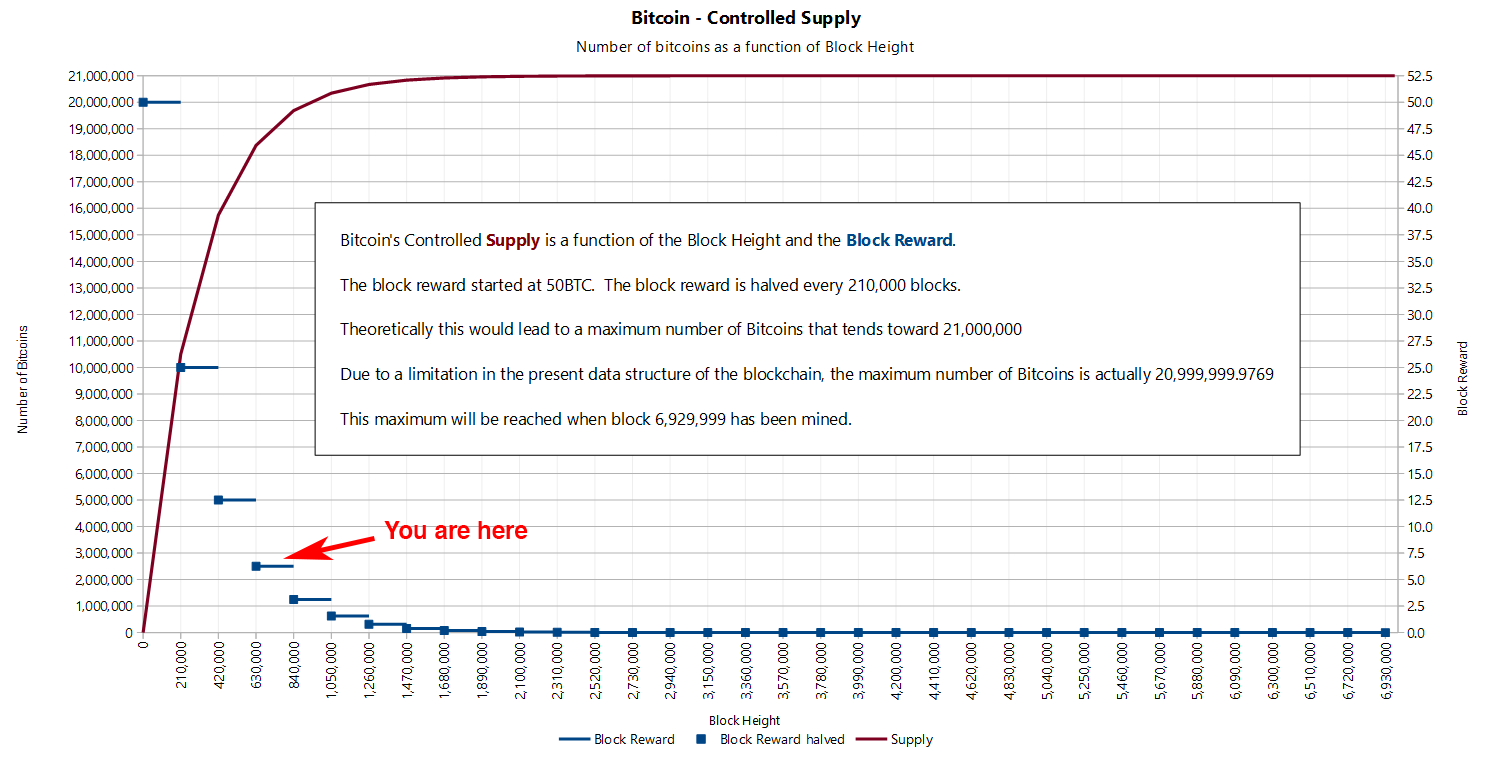
\includegraphics{assets/images/you-are-here.png}
  \caption{Bitcoin's controlled supply}
  \label{fig:you-are-here.png}
\end{figure}

Formulas, logarithmic functions and exponentials are not exactly
intuitive to understand. The concept of \textit{soundness} might be easier to
understand if looked at in another way. Once we know how much there is
of something, and once we know how hard this something is to produce or
get our hands on, we immediately understand its value. What is true for
Picasso's paintings, Elvis Presley's guitars, and Stradivarius violins
is also true for fiat currency, gold, and bitcoins.

The hardness of fiat currency depends on who is in charge of the
respective printing presses. Some governments might be more willing to
print large amounts of currency than others, resulting in a weaker
currency. Other governments might be more restrictive in their money
printing, resulting in harder currency.

Before we had fiat currencies, the soundness of money was determined by
the natural properties of the stuff which we used as money. The amount
of gold on earth is limited by the laws of physics. Gold is rare because
supernovae and neutron star collisions are rare. The \enquote{flow} of gold is
limited because extracting it is quite an effort. Being a heavy element
it is mostly buried deep underground.

The abolishment of the gold standard gave way to a new reality: adding
new money requires just a drop of ink. In our modern world adding a
couple of zeros to the balance of a bank account requires even less
effort: flipping a few bits in a bank computer is enough.

\begin{samepage}\begin{quotation}
\enquote{One important aspect of this new reality is that institutions like
the Fed cannot go bankrupt. They can print any amount of money that
they might need for themselves at virtually zero cost.}
\flushright -- Jörg Guido Hülsmann
\end{quotation}\end{samepage}

The principle outlined above can be expressed more generally as the
ratio of \enquote{stock} to \enquote{flow}. Simply put, the \textit{stock} is how much of
something is currently there. For our purposes, the stock is a measure
of the current money supply. The \textit{flow} is how much there is produced
over a period of time (e.g. per year). The key to understanding sound
money is in understanding this stock-to-flow ratio.

Calculating the stock-to-flow ratio for fiat currency is difficult, because how
much money there is depends on how you look at it.~\cite{wiki:money-supply} You
could count only banknotes and coins (M0), add traveler checks and check
deposits (M1), add saving accounts and mutual funds and some other things (M2),
and even add certificates of deposit to all of that (M3). Further, how all of
this is defined and measured varies from country to country and since the US
Federal Reserve stopped publishing \cite{web:fed-m3} numbers for M3, we will
have to make do with the M2 monetary supply. I would love to verify these
numbers, but I guess we have to trust the fed for now.

Gold, one of the rarest metals on earth, has the highest stock-to-flow
ratio. According to the US Geological Survey, a little more than 190,000
tons have been mined. In the last few years, around 3100 tons of gold
have been mined per year.~\cite{mineral-commodity-summaries}

Using these numbers, we can easily calculate the stock-to-flow ratio for
gold:

\begin{figure}
  \centering
  \begin{equation}
  \frac{190,000 t}{3,100 t} = ~ 61
  \end{equation}
  \caption{Stock-to-flow ratio of gold}
  \label{fig:stock-to-flow-gold}
\end{figure}

Nothing has a higher stock-to-flow ratio than gold. This is why gold, up to now,
was the hardest, soundest money in existence. It is often said that all the gold
mined so far would fit in two olympic-sized swimming pools. According to my
calculations\footnote{\url{https://bit.ly/gold-pools}}, we would need four. So
maybe this needs updating, or Olympic-sized swimming pools got smaller.

Enter Bitcoin. As you probably know, bitcoin mining was all the rage in
the last couple of years. This is because we are still in the early
phases of what is called the \textit{reward era}, where mining nodes are
rewarded with \textit{a lot} of bitcoin for their computational effort. We are
currently in reward era number 3, which began in 2016 and will end in
early 2020, probably in May. While the bitcoin supply is predetermined,
the inner workings of Bitcoin only allow for approximate dates.
Nevertheless, we can predict with certainty how high Bitcoin's
stock-to-flow ratio will be. Spoiler alert: it will be high.

How high? Well, it turns out that Bitcoin will get infinitely hard.

\begin{figure}
  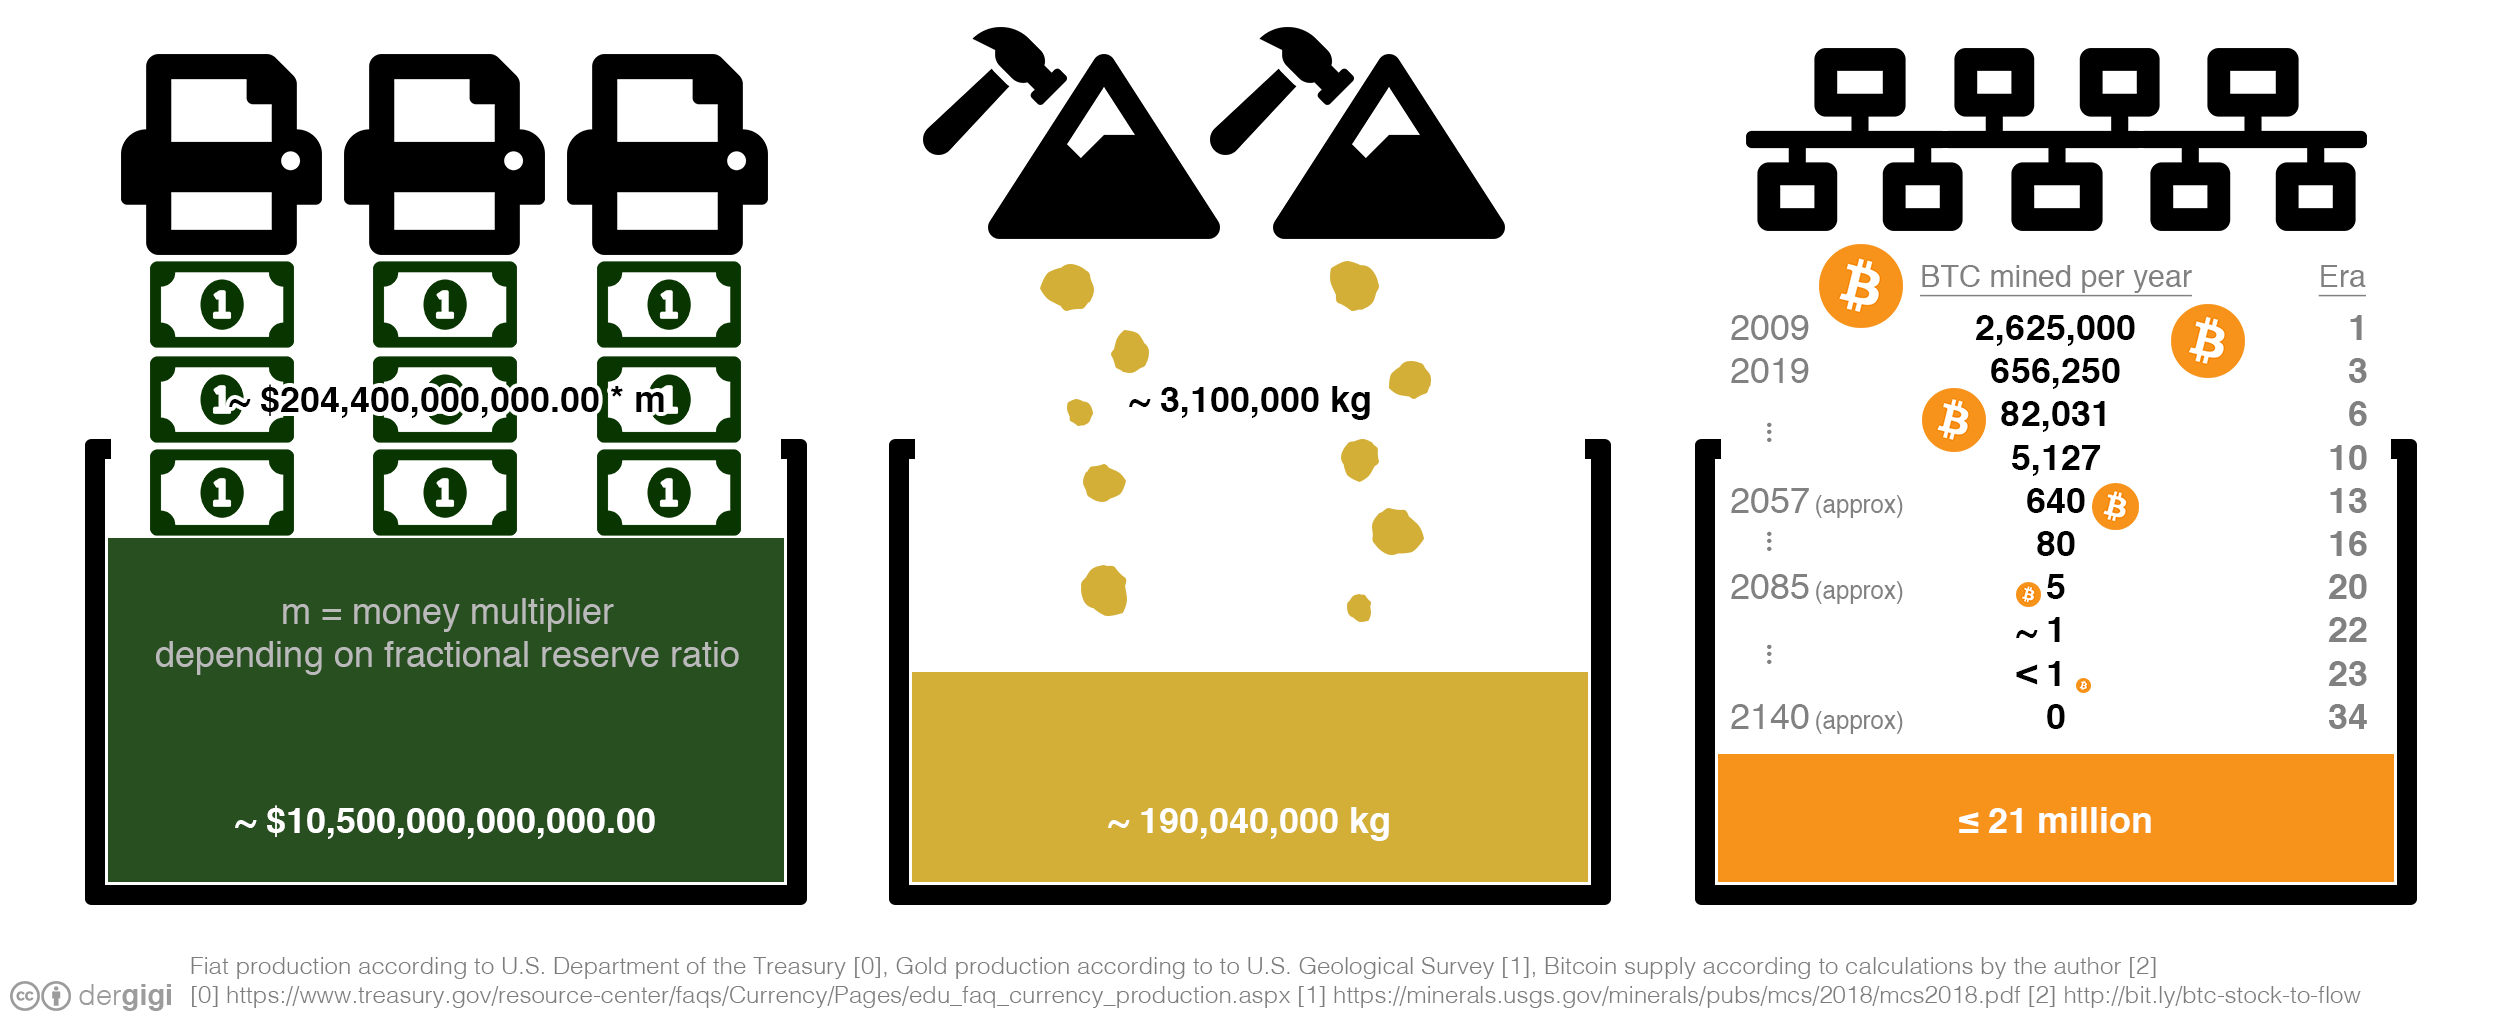
\includegraphics{assets/images/stock-to-flow-white-cc-by-sources.png}
  \caption{Visualization of stock and flow for USD, gold, and Bitcoin}
  \label{fig:stock-to-flow-white-cc-by-sources}
\end{figure}

Due to an exponential decrease of the mining reward, the flow of new
bitcoin will diminish resulting in a sky-rocketing stock-to-flow ratio.
It will catch up to gold in 2020, only to surpass it four years later by
doubling its soundness again. Such a doubling will occur 64 times in
total. Thanks to the power of exponentials, the number of bitcoin mined
per year will drop below 100 bitcoin in 50 years and below 1 bitcoin in
75 years. The global faucet which is the block reward will dry up
somewhere around the year 2140, effectively stopping the production of
bitcoin. This is a long game. If you are reading this, you are still
early.

\begin{figure}
  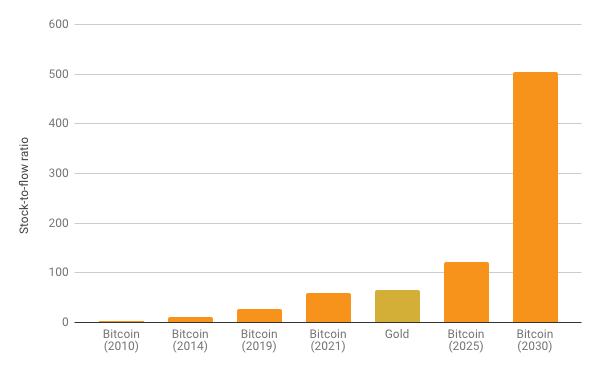
\includegraphics{assets/images/soundness-over-time.png}
  \caption{Rising stock-to-flow ratio of bitcoin as compared to gold}
  \label{fig:soundness-over-time}
\end{figure}

As bitcoin approaches infinite stock to flow ratio it will be the
soundest money in existence. Infinite soundness is hard to beat.

Viewed through the lens of economics, Bitcoin's \textit{difficulty adjustment}
is probably its most important component. How hard it is to mine bitcoin depends
on how quickly new bitcoins are mined.\footnote{It actually depends on how
quickly valid blocks are found, but for our purposes, this is the same thing as
\enquote{mining bitcoins} and will be so for the next 120 years.} It is the dynamic
adjustment of the network's mining difficulty which enables us to predict its
future supply.

The simplicity of the difficulty adjustment algorithm might distract
from its profundity, but the difficulty adjustment truly is a revolution
of Einsteinian proportions. It ensures that, no matter how much or how
little effort is spent on mining, Bitcoin's controlled supply won't be
disrupted. As opposed to every other resource, no matter how much
energy someone will put into mining bitcoin, the total reward will not
increase.

Just like $E=mc^2$ dictates the universal speed limit in our universe,
Bitcoin's difficulty adjustment dictates the \textbf{universal money limit}
in Bitcoin.

If it weren't for this difficulty adjustment, all bitcoins would have been mined
already. If it weren't for this difficulty adjustment, Bitcoin probably wouldn't
have survived in its infancy. It is what secures the network in its reward era.
It is what ensures a steady and fair distribution\footnote{Dan Held,
\textit{Bitcoin's Distribution was Fair}~\cite{distribution-was-fair}} of new
bitcoin. It is the thermostat which regulates Bitcoin's monetary policy.

Einstein showed us something novel: no matter how hard you push an
object, at a certain point you won't be able to get more speed out of
it. Satoshi also showed us something novel: no matter how hard you dig
for this digital gold, at a certain point you won't be able to get more
bitcoin out of it. For the first time in human history, we have a
monetary good which, no matter how hard you try, you won't be able to
produce more of.

\paragraph{Bitcoin taught me that sound money is essential.}

% ---
%
% #### Through the Looking-Glass
%
% - [Bitcoin's Energy Consumption: A Shift in Perspective][much energy]
%
% #### Down the Rabbit Hole
%
% - [The Ethics of Money Production][Jörg Guido Hülsmann] by Jörg Guido Hülsmann
% - [Mineral Commodity Summaries 2019][last few years] by the United States Geological Survey
% - [Bitcoin’s Distribution was Fair][fair distribution] by Dan Held
% - [Bitcoin's Controlled Supply][algorithmically controlled] on the Bitcoin Wiki
% - [Money Supply][how much money there is], [Speed of Light][universal speed limit] on Wikipedia
%
% <!-- Internal -->
% [much energy]: 
%
% [Fr. Bernard W. Dempsey, S.J.]: https://www.jstor.org/stable/29769582
% [Jörg Guido Hülsmann]: https://mises.org/sites/default/files/The%20Ethics%20of%20Money%20Production_2.pdf
% [stopped publishing]: https://www.federalreserve.gov/Releases/h6/discm3.htm
% [last few years]: https://minerals.usgs.gov/minerals/pubs/mcs/2018/mcs2018.pdf
% [my calculations]: https://www.wolframalpha.com/input/?i=volume+of+190000+metric+tons+gold+%2F+olympic+swimming+pool+volume
% [fair distribution]: https://blog.picks.co/bitcoins-distribution-was-fair-e2ef7bbbc892
%
% <!-- Bitcoin Wiki -->
% [algorithmically controlled]: https://en.bitcoin.it/wiki/Controlled_supply
%
% <!-- Wikipedia -->
% [how much money there is]: https://en.wikipedia.org/wiki/Money_supply
% [universal speed limit]: https://en.wikipedia.org/wiki/Speed_of_light#Upper_limit_on_speeds
% [alice]: https://en.wikipedia.org/wiki/Alice%27s_Adventures_in_Wonderland
% [carroll]: https://en.wikipedia.org/wiki/Lewis_Carroll
